\section*{Questions 7 and 8}

The last step of the parser is to recognize a formula $\Phi$. First we create a simple context free grammar for the formula. The productions are seen in table \ref{tab:Q7prod}. Again the first production is in order to read the whole file before parsing.

\begin{table}[H]
    \centering
    \begin{tabular}{|rl|}
        \hline
        F $\; \rightarrow$ &  phi \\
        phi $\; \rightarrow$ & 'TT' $|$ 'AP' $|$ 'AND[' phi '][' phi ']' $|$ 'NOT[' phi ']' \\
        phi $\; \rightarrow$ & 'EX[' phi ']' $|$ 'EF[' phi ']' $|$ 'AX[' phi ']' $|$ 'AG[' phi ']'\\
        \hline
    \end{tabular}
    \caption{The productions for creating a formula $\Phi$. The productions of phi are split up into two lines, to keep the table form getting too wide.}
    \label{tab:Q7prod}
\end{table}

Since the formula already is so recursively defined (without left-recursion) it is very simple to implement in antlr, as seen in table \ref{tab:Q7prod}

To create the abstract syntax tree, we again need to create some java classes: \texttt{Formula}, \texttt{Phi}, \texttt{ANDPhi}, \texttt{NOTPhi}, \texttt{EXPhi}, \texttt{EFPhi}, \texttt{AXPhi} and \texttt{AGPhi}. 

\texttt{Formula} is the head class (root of the parse tree) which takes \texttt{Phi} as a parameter in the constructor. \texttt{Phi} is the main class, which has the fields: String ap (atomic proposition) and \texttt{Phi} the formula from the children. All other classes extend \texttt{Phi}, and are used to control the evaluations of the ctl check (\texttt{ANDPhi} is a special case since it contains two \texttt{Phi} fields, otherwise similar). The complete code for the formula as implemented in antlr3.5 can be seen in the appendix.

The \texttt{evaluate} methods of the different formula classes are all created using the Mandatory Assignment 2. By evaluating the ctl checks in the abstract syntax tree for the formula, we are sure that the sequence of checks are performed correctly. The transition system is delivered from the EnvironmentTS (the environment for evaluating the transition system) directly to EnvironmentF (the environment for evaluating the formula). An example of the abstract syntax is seen in the appendix.


When everything is set up and compiled, we are able to feed the program two arguments: 1) The file containing the transition system 2) the formula to be checked. The program then returns all states which fulfill the formula on the given transition system.

Some examples of program outputs are shown in figure \ref{fig:Q8ex}. This figure only shows the program output, consisting of the complete system followed be the resulting states satisfying the given formula. For reference, the used formulas are shown in the subfigure's captions.


\begin{figure}[H]
    \begin{subfigure}{0.49\textwidth}
        \centering
        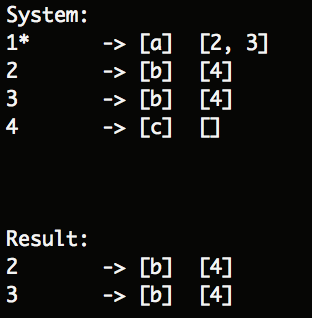
\includegraphics[width=0.5\textwidth]{fig/Q8example1}
        \caption{EX[c]}
        \label{fig:Q8ex1}
    \end{subfigure}
    \begin{subfigure}{0.49\textwidth}
        \centering
        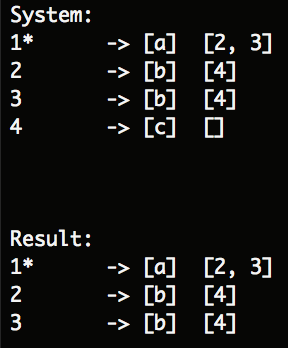
\includegraphics[width=0.5\textwidth]{fig/Q8example2}
        \caption{EF[b]}
        \label{fig:Q8ex2}
    \end{subfigure}
    \newline
    \begin{subfigure}{0.49\textwidth}
        \centering
        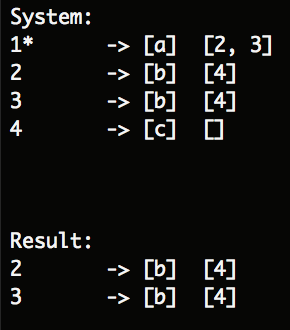
\includegraphics[width=0.5\textwidth]{fig/Q8example3}
        \caption{AND[EX[AG[c]]][AX[c]]}
        \label{fig:Q8ex3}
    \end{subfigure}
    \begin{subfigure}{0.49\textwidth}
        \centering
        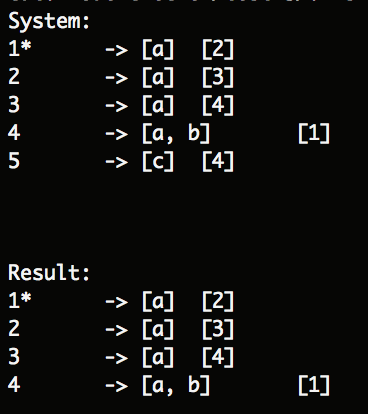
\includegraphics[width=0.5\textwidth]{fig/Q8example4}
        \caption{AG[a]}
        \label{fig:Q8ex4}
    \end{subfigure}
    \caption{Examples of transition systems checked with ctl formula.}
    \label{fig:Q8ex}
\end{figure}

If we look at figure \ref{fig:Q8ex}, we see that the a)-c) use the same transition system, and d) use a circular transition system with a protrusion. These two transition systems are sketched in figure \ref{fig:Q8sketch}.

\begin{figure}[H]
    \begin{subfigure}{0.49\textwidth}
        \centering
        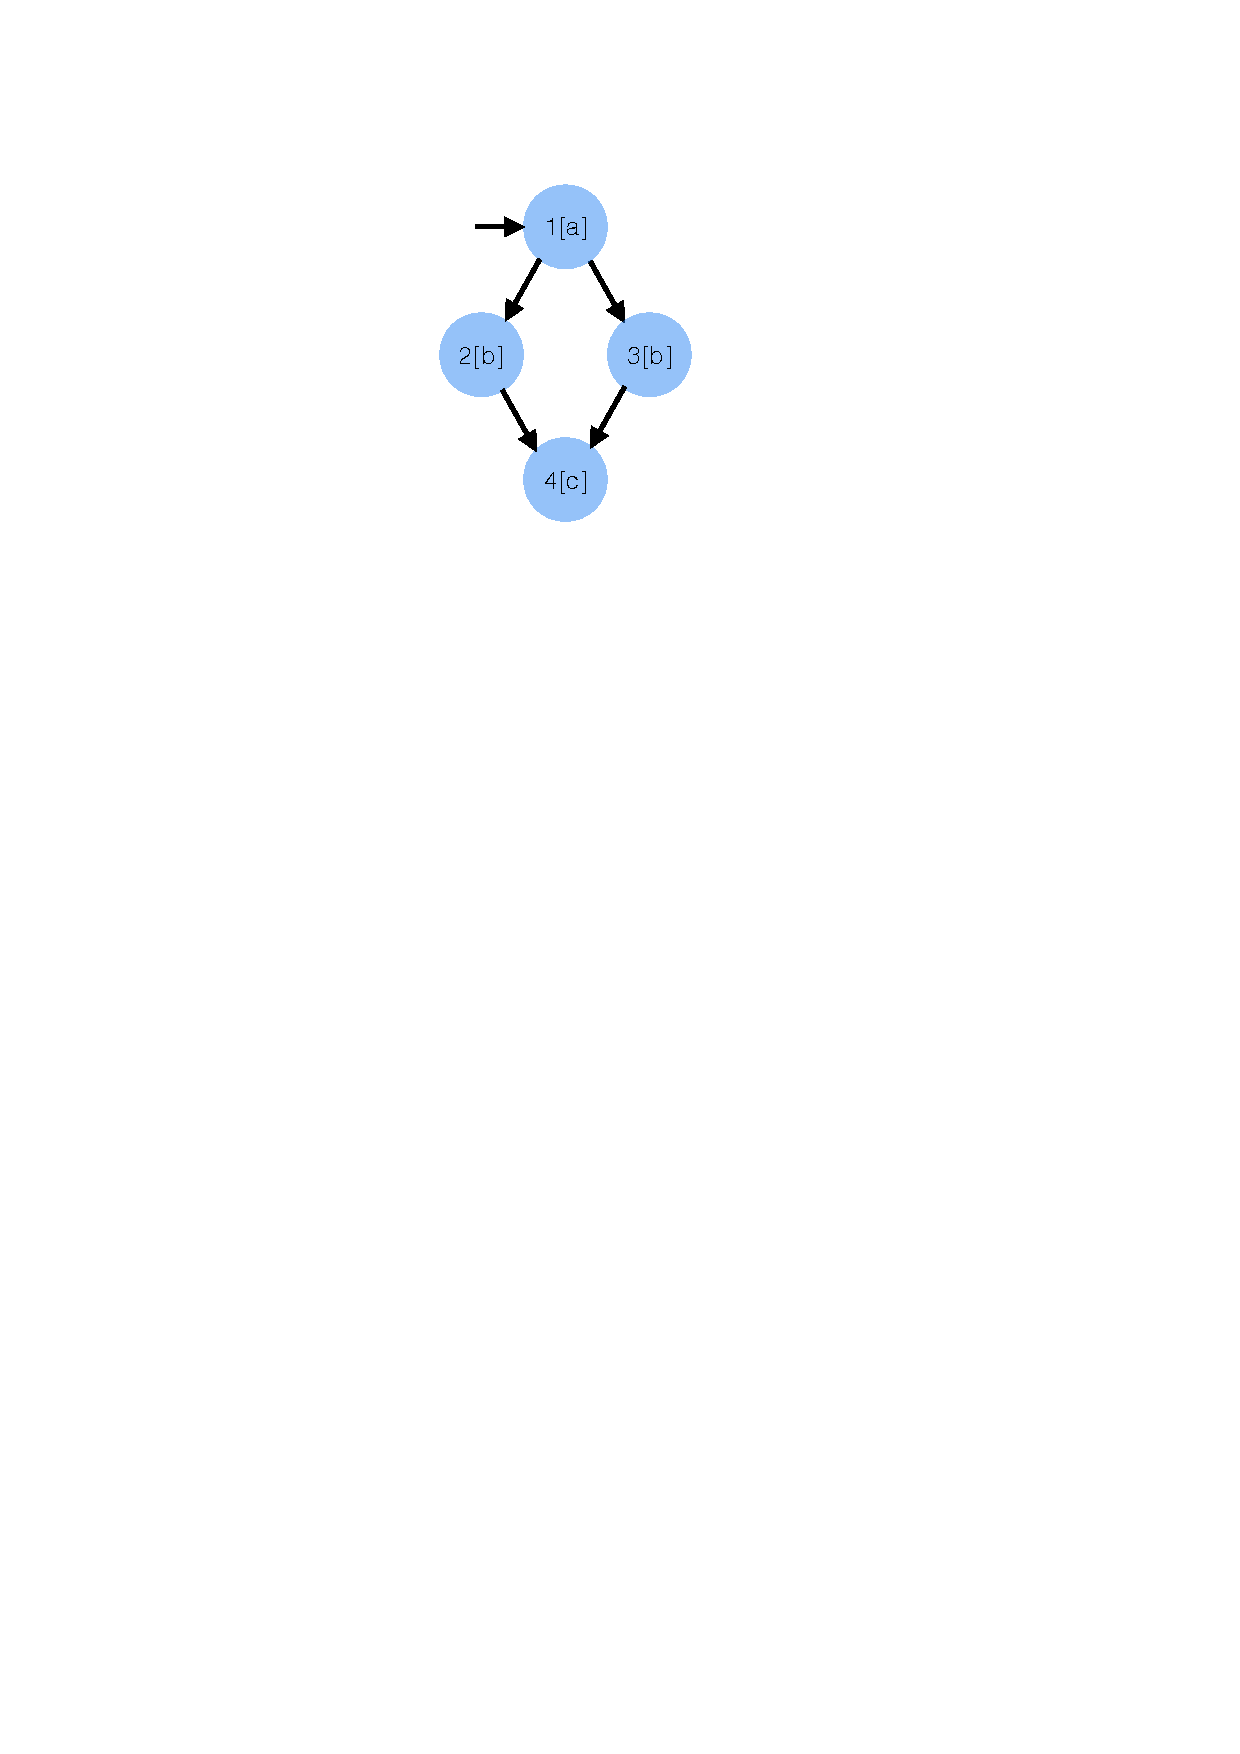
\includegraphics[width=0.5\textwidth]{fig/TS1}
        \caption{Transition system for figure \ref{fig:Q8ex} a)-c).}
        \label{fig:TS1}
    \end{subfigure}
    \begin{subfigure}{0.49\textwidth}
        \centering
        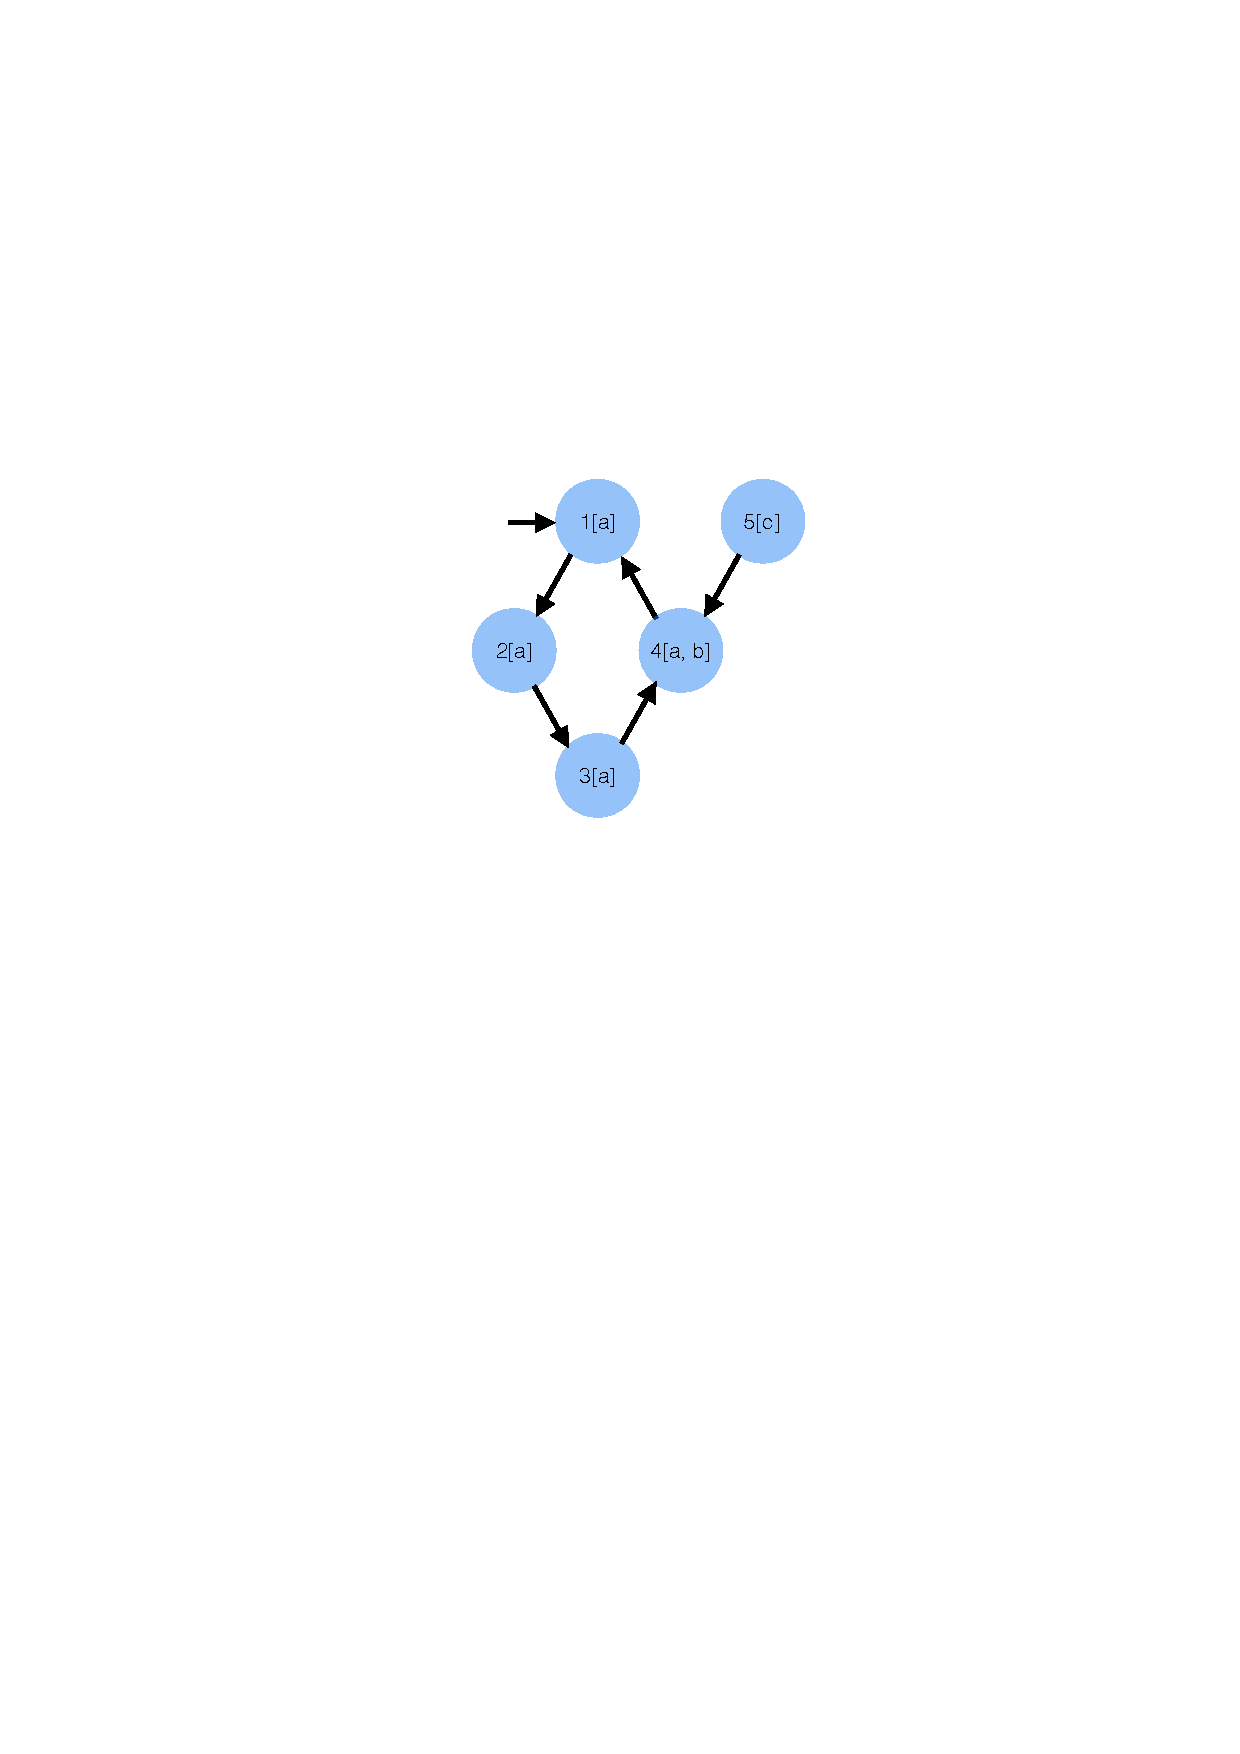
\includegraphics[width=0.65\textwidth]{fig/TS2}
        \caption{Transition system for figure \ref{fig:Q8ex} d).}
        \label{fig:TS2}
    \end{subfigure}
    \caption{Sketches of the transition systems used in figure \ref{fig:Q8ex}}
    \label{fig:Q8sketch}
\end{figure}

With figure \ref{fig:Q8ex} and figure \ref{fig:Q8sketch} we can check the output of the program for each example.

\subsubsection*{Example a):}
This example uses the formula EX[c]. All states where it is possible to go to a state (in one step) with atomic proposition c are states 2 and 3. This matches the output of the program.

\subsubsection*{Example b):}
This example uses the formula EF[b]. All states where it is possible to go to a state (in any amount of steps) with atomic proposition b are states 1, 2 and 3. This matches the output of the program.

\subsubsection*{Example c):}
This example uses the formula AND[EX[AG[c]]][AX[c]]. We will break this formula up into parts. The only state satisfying AG[c] is state 4. The states satisfying EX[$\{4\}$]\footnote{We here use the notation from the \texttt{Sat} function from Flemming Nielsens notes (chapter 5, bonus material).}, are states 2 and 3. The only states satisfying AX[c] are states 2 and 3, so the formula AND[$\{2, 3\}$][$\{2, 3\}$] is satisfied by the states 2 and 3. This matches the output of the program.

\subsubsection*{Example d):}
This example uses the formula AG[a]. Compared to the previous example, this is an easy one. The states satisfying AG[a] are the states confined within the circle of the transition system. This matches the output of the program.

\vspace{5mm}
This concludes that our parser is correct and is able to read transition systems and formulas from files. Creating abstract syntax trees for the system and formula. Returning all states which satisfy the formula on the given transition system.
